%!TEX root = ../Thesis.tex
\section{Beschreibung des Projektverlaufs}

\subsection{Tatsächliche Aufgabenverteilung im Team (tabellarisch)}

\subsection{Teammeeting-Protokolle}



\subsection{Projekttagebücher aller Teammitglieder (tabellarisch)}

\subsubsection{Tom Bockhorn}

\subsubsection{Hendrik Falk}

\subsubsection{Dennis Gentges}

\subsubsection{Getuart Istogu}

\subsubsection{Jannis Keienburg}

\subsubsection{Tim Jonas Meinerzhagen}

\subsubsection{Khang Pham}

\subsubsection{Tim Schwenke}

\subsection{Beschreibung von Problemen}

\subsubsection{Softwareentwicklung im Team [Schwenke]}

Schon kurz nach der initialen Erstellung des Git-Repositories und des Projekts in Android-Studio hat sich die Frage gestellt, wie man in einem acht Mitglieder starkem Team produktiv an einer einzelnen Code-Basis arbeiten soll. Hat man ein Quellcodeverzeichnis alleine für sich reichen zumeist um die drei aktive (also nicht \textit{stale}) Branches aus. Das wäre zunächst der \code{Master}-Branche, welcher die Wurzel des Verzeichnisses darstellt und – gerade, wenn Ansätze wie CI/CD verfolgt werden – die produktiven oder zumindest lauffähigen Versionen eines Projekts enthält. Im \code{Development}-Branch hingegen findet die Entwicklung statt. Hier ist es üblich, dass das Projekt zum Zeitpunkt einzelner Commits Fehler enthält und nicht lauffähig ist. Sobald ein Entwickler der Meinung ist, dass der Stand in \code{Development} veröffentlicht werden kann, wird \code{Development} in \code{Master} vereint. Wichtig zu betonen ist hier, dass dies keine feste Regel ist, sondern eher dem allgemeinen Workflow entspricht. In einem großen Team ist ein solcher Arbeitsablauf nicht mehr möglich. So müssen mehrere Entwickler parallel an dem Projekt arbeiten. Verwendet man nun das System aus zwei Branches, wird es sehr schnell zu Merge-Konflikten kommen, die die Entwickle dazu zwingen sich mehr mit der korrekten Zusammenführung als der eigentlichen Entwicklung zu beschäftigen, sofern sie ihren lokalen Arbeitsbereich aktuell halten wollen. Die nächstliegende und ebenfalls problematische Alternative ist es nur bei Fertigstellung von Funktionen, die meist aus mehreren Commits zusammengesetzt sind, das lokale Quellcodeverzeichnis mit dem Remote zu synchronisieren. Mit dieser Herangehensweise verpasst man unter Umständen große Fortschritte im Gesamtprojekt. Die lokale Version ist plötzlich nicht mehr lauffähig und muss aufwändig angepasst werden. Deswegen haben wir uns in diesem Projekt für den Gitflow-Workflow entschieden. Grafisch dargestellt ist dieser beispielhaft in der folgenden Grafik.

\begin{figure}[h]
	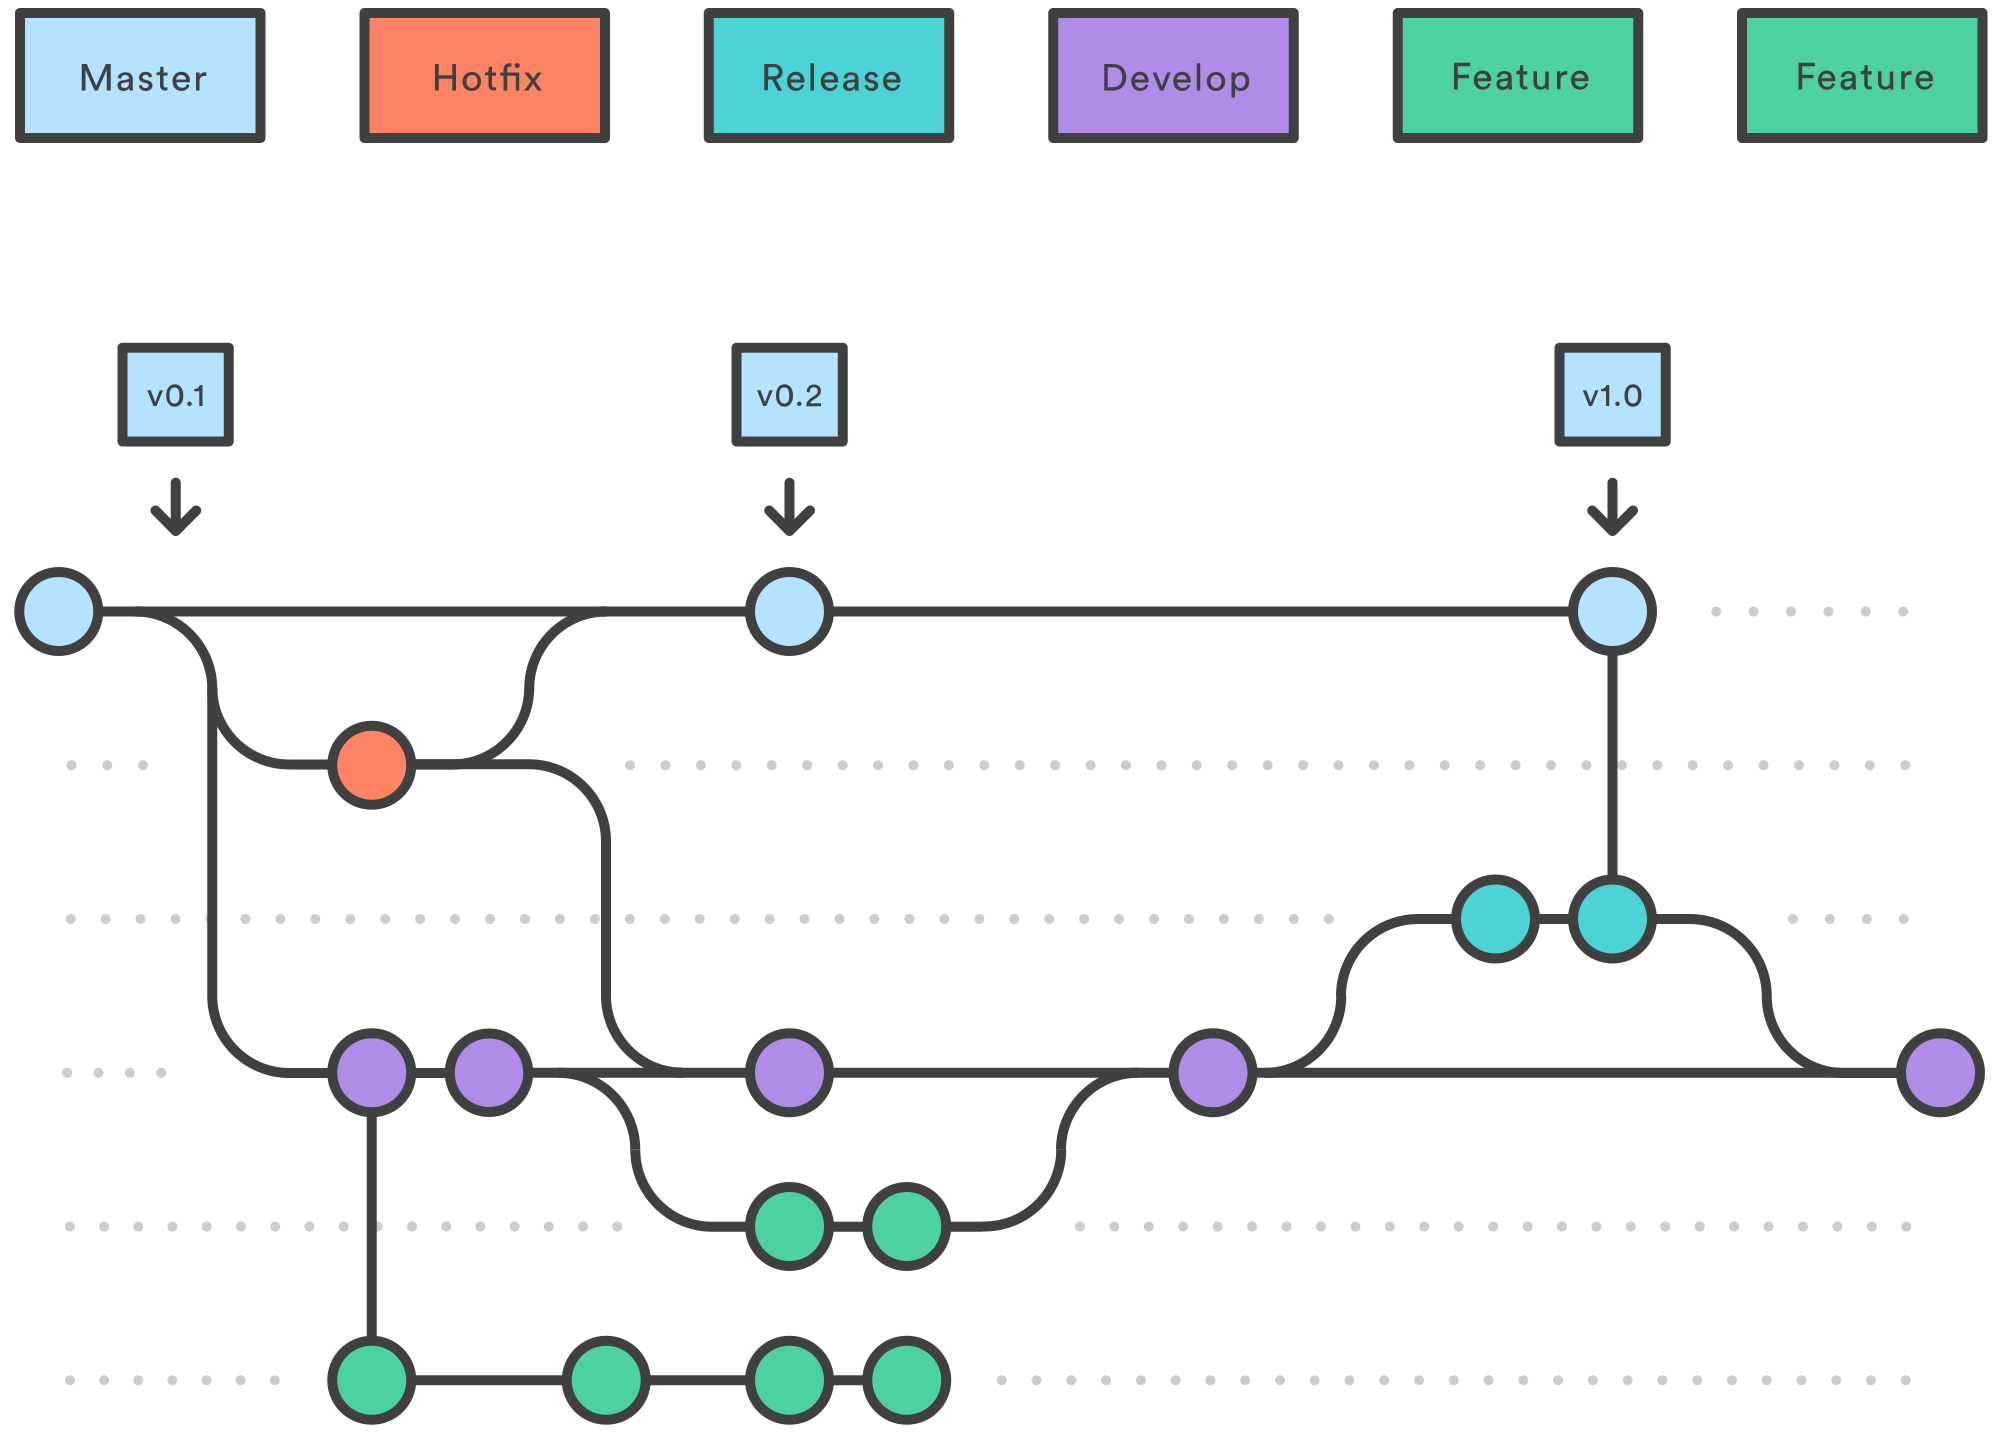
\includegraphics[width=\columnwidth]{img/gitflow}
	\caption[Gitflow]{Gitflow\footnotemark}
\end{figure}
\footnotetext{\cite{atlassian2020}}

Der Gitflow-Workflow definiert ein strenges Branching-Model und gibt jedem Typ von Branch (lediglich differenziert durch ihre Namen) eine spezifische Rolle. \code{Master} wird verwendet, um die Release-History festzuhalten. Hier finden sich Versionen des Projekts, die lauffähig sind und für sich alleine stehen (können). \code{Development} fungiert ähnlich wie \code{Master}, nur enthält es die gesamte Entwicklungshistorie des Projekts. Nun kommen die sogenannten \code{Feature}-Branches ins Spiel, die beliebig weiter untergliedert werden können. Benannt werden Features hierarchisch. In unserem Projekt haben wir folgende zwei Gruppen von Feature-Branches: 

\texttt{feature/backend/<konkretes-feature>}

\texttt{feature/frontend/<konkretes-feature>}

Jedes Feature wird einem Verantwortlichen zugeteilt und wird meist auch von diesem bearbeitet. Sobald ein Feature fertig ist, wird es in \code{Development} zusammengeführt. Somit werden die Abstände zwischen Zusammenführungen verringert und der Arbeitsablauf wird einfacher. Schließlich gibt es auch noch einen Hotfix-Branch, für dringende Änderungen.

Im Laufe der Entwicklung haben sich die Vorteile dieser Herangehensweise für das Team deutlich gezeigt. Unterschiedliche Features konnten, nachdem eine grundlegende Programmarchitektur umgesetzt wurde, meist ohne Probleme zusammengeführt werden. 